\documentclass[12pt,titlepage,twoside]{report}
% font
\usepackage{dejavu}
\usepackage{sectsty}
\allsectionsfont{\sffamily}
% language stuff
\usepackage{german, ngerman}           % deutsche Überschriften etc.
\usepackage[utf8]{inputenc} % direkte Einbgabe von Umlauten
% miscellaneous
\usepackage{graphicx}         % graphics
\graphicspath{{grafiken/}}
\usepackage[german]{fancyref}
\usepackage{hhline}           % double lines in tables
\usepackage{amsfonts}         % real numbers etc.
\usepackage[rightcaption]{sidecap} % figure captions on the right (optional)
\usepackage{hyperref}         % for URLs
\usepackage{listings}         % for code samples
\usepackage{fancyhdr}         % for header line
\usepackage[backend=biber, style=authoryear-icomp]{biblatex}
\addbibresource{literatur.bib}
% \usepackage{natbib}
% Hier bei Bedarf die Seitenränder einstellen

\usepackage[printonlyused]{acronym}

\usepackage{algorithm}

% Kopf- und Fußzeile
\fancyhead{} % clear all header fields
\fancyhead[RO,LE]{\leftmark}

\title{Arbeit}
\author{Alexander Martin}
\date{August 2021}

\begin{document}

\begin{titlepage}
  \begin{center}
    {\Large\bf Entwurf und Implementierung einer generischen Ingestion-Schnittstelle mit Versionierung für Data-Lake-Systeme}\\[2cm]

    {\bf Masterarbeit}\\
    zur Erlangung des Grades {\em Master of Science}\\[1cm]

    an der\\
    Hochschule Niederrhein\\
    Fachbereich Elektrotechnik und Informatik\\
    Studiengang {\em Informatik}\\[2cm]

    vorgelegt von\\
    Alexander Martin\\
    1018332\\[3cm]
    Datum: \today\\[2cm]

    Prüfer: Prof.~Dr.~rer.~nat.~Christoph Quix\\
    Zweitprüfer: Sayed Hoseini,~M.Sc.

  \end{center}
\end{titlepage}
\newpage
\include{unabhänhigkeit}
\newpage
\section*{Zusammenfassung}

Heutzutage spielen Daten eine immer wichtiger Rolle.
Durch den vermehrten Einsatz von IoT-Geräten und moderne Cloud-Speicher-Lösungen, wächst die Zahl an anfallenden Daten vielen Firmen und Forschungseinrichtungen stetig.
Mit steigenden Datenmengen und der diversen Strukturen der Daten ist deren Verwaltung ein komplexes Thema geworden.
Diese Arbeit befasst sich mit der technischen Herausforderung Daten aus verschiedensten Quellen zu Verwalten.
Als Lösung hierfür wurden Data-Lake-Systeme vorgeschlagen.
Im Kontext des HIT-Institut der Hochschule Niederrhein, wurde ein Prototyp für einen Data-Lake entwickelt.
In dieser Arbeit wird eine Schnittstelle entwickelt, über die Benutzer Daten aus unterschiedlichen Quellen in dieses System laden können.
Dabei werden Metadaten über die Datenquellen gesammelt.
Mit der Schnittstelle ist es auch möglich, die geladenen Daten zu versionieren, um weiter Verarbeitungen effizienter zu machen.

\section*{Abstract}

In todays world data play an important role.
The amount of data in comapnies and research facilities is growing due to the increasing use of IoT-devices and modern Cloud-Storage-Solutions.
With the bigger amount of data and their varying structures the data management got more complex.
This thesis takes on the technical challenge of managing data from different sources.
Data lakes are a proposed solution for this problem.
A prototype for a data lake was developed at the HIT-institute at the Hochschule Niederrhein.
This thesis devolopes an interface for users to ingest data from diffenrent sources to the system.
The interface collects metadata about the data sources.
It is also capable of saving data with versioning to make further processing more efficient.
\newpage

\pagestyle{fancy}
\tableofcontents
\newpage

\chapter{Einleitung}

\section{Die Motivation}
In der heutigen Zeit spielen Daten in der Welt eine immer größere Rolle.
In \textit{Rethink Data Report 2020} \textcite{rethink_data_2020} wurde eine Studie durchgeführt, die eine Steigerung von 42\% der Menge an anfallenden Daten pro Jahr prognostiziert.
Dies wird unter anderem auf den vermehrten Einsatz von IoT-Geräten, immer ausführlicheres Analysieren von Daten und die einfacher werdende Anwendung von Cloud-Speichern zurückgeführt.
Dabei besteht die Herausforderung, Daten in verschiedensten Formaten in großen Mengen zu verwalten und zu verwenden.

Ein Lösungansatz für dieses Problem sind Data-Lake-Systeme.
Data-Lake-Systeme sind zentrale Datenspeicher, die strukturierte, semi- und unstrukturierte Daten in ihrem Rohformat speichern.
Mit Hilfe von Metadaten bietet ein Datalake Schnittstellen zur Datenanalyse und -abfrage.
Dabei funktioniert das System nach dem Schema-On-Read oder auch ELT (Extrahieren Laden Transformieren) Prinzip.
Das bedeutet, dass die Daten wie bereits erwähnt im Rohformat im Data Lake gespeichert werden und erst nach dem Laden ein entsprechendes Schema angewendet wird.

Es gibt bereits viele Anbieter, die fertige Data-Lake-Systeme anbieten.
Dabei ist jedoch ein Nachteil, dass sie häufig nur in der (Cloud-)Infrastruktur des Anbieters (z.B. Microsoft Azure\footnote{https://azure.microsoft.com/}, Amazon Web Services\footnote{https://aws.amazon.com/}) verfügbar sind und sich ihrere Architektur nach diesen Diensten richtet.
Daher wird in dieser Arbeit eine Schnittstelle für die Ingestion, also das Laden der Daten in das Data-Lake-System, entwickelt, die in einem platform unabhängigen Data-Lake-System Anwendung finden soll.

\section{Der Aufbau}
Am Anfang wird auf die Ziele eigengangen, die Schnittstelle erreichen soll.
Aus diesen Zielen werden dann konkrete Anforderungen an die Entwicklung abgeleitet.
Im zweiten Kapitel wird das System der Schnittstelle entwickelt, ohne dabei auf konkrete Details, wie zum Beispiel Programmiersprachen, einzugehen.
Hier geht es mehr um die Architektur und das Design, das benötigt wird um alle Anforderunegn abzudecken.
Danach wird die Umsetzung beschrieben.
Hierbei spielt vorallem das bereits exisitierende Data-Lake-System, in dem die Ingestion-Schnittstelle integriert werden soll, eine große Rolle.
Zum Schluss wird die Ingestion-Schnittstelle evaluiert und ein Ausblick auf mögliche weitere Arbeiten gegeben.

\section{Das Existierende System}
In dem Masterprojekt \textit{Development of a Data Lake System} \parencite{datalake_proj} an der Hochschule Niederrhein wurde bereits eine Data-Lake-System-Prototyp entwickelt.
Das System ist eine monolithische Client-Server-Anwendung.
Es besteht aus einer REST-API, die zur Interaktion mit dem Data-Lake-System verwendet wird und einem Web-Frontend.
Außerdem können durch einfach Anpassungen der Server-Anwendung beliebige Datenspeicher in das Data-Lake-System integriert werden.

Als Basis wird \textit{Apache Spark}\footnote{https://spark.apache.org/} verwendet.
\textit{Apache Spark} ist eine Plattform, um Analyse auf großen Datenmengen aus zu führen.
Außerdem gibt es Schnittstellen für \textit{Scala, Java und Python} und es wird auch die Verarbeitung von Datenströmen und maschinelles Lernen unterstützt \parencite{spark}.

Der Server ist in \textit{Python} geschrieben und verwendet das Framework \textit{Flask}\footnote{https://palletsprojects.com/p/flask/} um eine REST-API bereitzustellen, über die mit dem Data Lake interagiert werden kann.
Dabei werden über die API \textit{JSON}-Objekte ausgetauscht, so dass die API client-unabhängig verwendet werden kann.
Der Client des Projekts ist eine Webanwendung, die mit \textit{Angular}\footnote{https://angular.io/} umgesetzt wurde.

\section{Verwandte Arbeiten}

\chapter{Ziel und Anforderungen}
In diesem Kapitel werden die Ziele und Anforderungen für die Entwicklung ermittelt.
Dazu wird zuerst die Zielsetzung beschrieben.
Diese soll aber nur als Grundlage für die Anforderungen dienen, weshalb die Ziele nicht detailiert erklärt sind.
Das geschieht im zweiten Teil, in dem dann auch die Anforderungen abgeleitet werden.

\section{Zielsetzung}
Allgemein formuliert ist das Ziel eine Ingestion-Schnittstelle, die in der Lage sein soll, Daten in verschiedenen Formaten quellenunabhängig zu laden und in unterschiedlichen Speichern abzulegen.
Zusätzlich soll die Möglichkeit gegeben werden Daten kontinuierlich nach zu laden und optional diese zu Versionieren, so dass man die Änderungen von Daten nachvollziehen kann.
Dies alles soll, im Gegensatz zur existierenden Schnittstelle aus dem Prototypen, ohne Anpassungen im Server-Code möglich sein.

Wie bereits erwähnt, ist der Data-Lake-System-Prototyp eine monolithische Anwendung.
Das bedeutet, dass die gesamte Anwendung als komplett Lösung in einem Programm entwickelt und bereit gestellt wird.
Solche Ansätze sind Anfangs leichter umzusetzen, haben aber größere Nachteile in Bereichen wie Fehlertoleranz und Wartbarkeit.
Daher soll für die Ingestion-Schnittstelle der Microservice-Ansatz verfoglt werden.
Hierbei werden die Funktionalitäten und Aufgaben auf mehrere kleinere Anwendungen aufgeteilt.
Das hat den, wie von \textcite{microservices} dargestellt, mehrere Vorteile.
Die Wartung fällt bei mehreren kleinen Programmen leichter, da sie übersichtlicher und verständlicher sind.
Bei Fehlerfunktionen einzelner Mircoservices faällt außerdem nicht die komplette Anwendung aus, sondern nur die Funktion, für die der Service zuständig war.
Zuletzt ist es einfacher bestimmte Aspekte der Software zu skalieren und bei Updates bleibt eine höhere Verfügbarkeit, da nur ein kleiner Teil des Systems neu gestartet werden muss.

\section{Anforderungen}
Aus den oben genannten Zielen lassen sich jetzt genauere Anforderungen entwickeln, die die Ingestion-Schnittstelle erfüllen soll.
Dazu werden nachfolgend die einzelnen Ziele in Abschnitte aufgeteilt und die dazugehörigen Anforderungen festgehalten.
In der Evaluierung kann dann überprüft werden, ob alle Anforderung durch das Ergebniss erfüllt werden.
Die Unterkapitel sind so aufgebaut, dass erst eine genauere Erklärung für das Ziel gegeben wird und dann in einzelnen Paragraphen die Anforderungen nummeriert aufgelistet werden.

\subsection{Quellen- und Formatunabhänigkeit}
Es soll die Möglichkeit gegeben werden, Daten aus jeder beliebigen Quelle in das System zu integrieren.
Dazu muss die Schnittstelle sowohl in der Lage sein direkt Daten entgegen zu nehmen als auch aus anderen Systemen zu extrahieren.
Unter System wird hierbei jedoch nicht nur eine Datenbank verstanden, sonder es können unter anderem auch Dateien, APIs oder Datenströme gemeint sein.
Ebenso soll es möglich sein, den Speicher im Data-Lake-System für die Daten auszuwählen.
Da im Prototypsystem \textit{Apache Spark} verwendet wird, wird die Funktion, Daten in verschiedensten Formaten zu laden und zu speichern als gegeben betrachtet.

\paragraph{ANF\_01}
Die Schnittstelle muss in der Lage sein Quelldaten entgegen zu nehmen, die an das Data-Lake-System gesendet werden.
Diese müssen so verwaltet werden, dass sie über \textit{Apache Spark} gelesen werden können.

\paragraph{ANF\_02}
Da \textit{Apache Spark} nicht von sich aus in der Lage ist, alle Datenformate zu verstehen, muss es möglich sein die \verb|SparkSession| mit benötigten Packeten zu erweitern.

\paragraph{ANF\_03}
Für die Unterstützung verschiedenster Quell- und Zielsystem verwendet \textit{Apache Spark} zum Lesen und Speichern von Dateien eine Format-Parameter und Optionen.
Diese sollen komplett konfigurierbar sein um alle Systeme verwenden zu können.

\paragraph{ANF\_04}
Einige Funktionalitäten, wie zum Beispiel das Ausführen einer Reihnfolge von Abfragen an eine Programmierschnittstelle können nicht durch \textit{Apache Spark} abgedeckt werden.
Daher soll es eine Möglichkeit geben der Ingestion-Schnittstelle eigenen Programmcode mit zu geben, der diese Funktionen abdeckt.

\subsection{Kontinuierliches Laden}
Da Daten sich mit der Zeit ändern, soll die Ingestion-Schnittstelle in der Lage sein, neue Daten aus einer Datenquelle, die bereits ingested wurde, erneut zu laden.
Hierfür sollen drei verschiedene Optionen zu Auswahl stehen.

\paragraph{ANF\_05}
Es soll möglich sein, Datenströme in das Data-Lake-System zu integrieren und als Quelle für kontinuierliche Daten zu verwenden.

\paragraph{ANF\_06}
Um aktuelle Daten aus Datenquellen, die nicht über einen Datenstrom verfügen, zu integrieren, soll es eine zeitgesteuerte wiederholte Ausführung geben.

\paragraph{ANF\_07}
Zur Ermöglichung einer unregelmäßigen wiederholten Inegstion einer Datenquelle, soll es einen API-Endpunkt geben, über den eine Ingestion gestartet werden kann.
Dieser soll auch dazu verwendet werden können, externe Systeme, wie eigene Change-Data-Capture-Lösungen, als Auslöser für eine Ingestion anbinden zu können.

\paragraph{ANF\_08}
Um Konflikte durch gleichzeitig laufende Ingestions der selben Datenquelle zu vermeiden, soll das System sicher stellen, dass für eine Datenquelle immer nur eine Ingestion läuft.

\subsection{Datenversionierung}
Durch das kontinuierliche Laden von Daten, entstehen laufend neue Versionen eines Datensatzes einer Datenquelle.
Diese Veränderungen der Daten können in vielen Anwendungsfällen bei der Auswertung von Interesse sein.
Dabei gibt es zwei verschiedene Wege, diese Daten in das System einzupflegen.
Einmal die Verwendung von Change-Data-Capture-Lösungen, die bereits in den Daten die Informationen über Änderungen enthalten und zweitens kann einfach der aktuelle Stand eines Datensatzes erneut geladen werden.

\paragraph{ANF\_09}
Daher soll das System eine Möglichkeit bieten das Einfügen, Aktualisieren oder Löschen von Daten festzuhalten und zur Abfrage zur Verfügung zu stellen.
Außerdem sollen damit auch die Daten zu bestimmten Zeitpunkte rekonstruierbar sein.

\paragraph{ANF\_10}
Die Ingestion-Schnittstelle soll Daten aus externen Change-Data-Capture-Systemen in den Datensatz und die Datenversionierung einer Datenquelle einpflegen können.

\paragraph{ANF\_11}
Da neben den Change-Data auch das laden eines aktuellen Datensatzes integriert werden kann, soll ein allgemeines Vorgehen entwickelt werden, diese auch in die Datenversionierung einpflegen zu können.

\subsection{Architektur}
Wie bereits geschrieben, soll die Inegstion-Schnittstelle in einer Mircoservice-Arichtektur umgesetzt werden.
Außerdem wird eine Schnittstelle für die Interaktion mit dem System benötigt.
Daraus ergeben sich folgende Anforderungen, an die Architektur.

\paragraph{ANF\_12}
Die Interaktions-Schnittstelle mit dem System soll eine REST-API sein, die keine Konflikte mit dem aktuellen Prototypen erzeugt.

\paragraph{ANF\_13}
Die Aufgaben der einzelnen Mircoservices müssen klar getrennt werden.
Die Überschneidungen zwischen den Mircoservices sollten so gering wie möglich gehalten werden.

\paragraph{ANF\_14}
Für die Kommunikation zwischen den Microservices soll eine einnheitliche Lösung entwickelt werden.
Diese soll es auch ermöglichen neue Mircoservices einfach in die Architektur einzubringen.



\chapter{Entwicklung}
In diesem Kapitel werden die einzelnen Komponenten, die für eine komplette Ingestion notwendig sind entwickelt.
Nach \citeauthor{DL-Ing-Mgmt} ist der Ingestion-Prozess eines Data-Lake-Systems, als erster Schritt im Lebenszyklus der Daten, maßgebend dafür, wie gut die Daten später verwendet und verarbeitet werden können.
Um diese Aufgabe so gut wie möglich zu erfüllen, wurden im vorherigen Kapitel bereits die Anforderung festgelegt.
Daraus ergeben sich die drei Inhaltlichen Bereiche, nach denen die weiter Entwicklung aufgeteilt ist.

Der erste ist die Ingestion.
Diese beschreibt das erfassen von Informationen über eine Datenquelle und das Laden der Daten aus der Datenquelle.
Dabei werden die Daten noch nicht intern im Data Lake wieder abgelegt sondern existieren nur flüchtig im Arbeitsspeicher.

Die Deltaerkennung ist dafür zuständig die Unterschiede zwischen den geladenen Daten im Arbeitsspeicher und den aktuellen Daten aus dem internen Data Lake Speicher zu finden.
Aus diesen Unterschieden sollen die Änderungsdaten erstellt werden, die dann bei der weiteren Verarbeitung verwendet werden können.

Der dritte Bereich ist das Speichern von Daten in einem vordefinierten als auch in einem frei bestimmbaren Speichersystem zählt.
Der Unterschied dabei ist, dass im vordefinierten Speicher die Datenversionierung durch das Data-Lake-System unterstützt wird, während dies bei frei wählbaren nicht der Fall ist.

\section{Architektur}
\label{sec:arch}

Zu Anfang ist es sinnvoll, die Architektur des Systems festzulegen.
Diese bestimmt, welche Komponenten und Microservices entwickelt und verbunden werden müssen.
Der erste Schritt dabei ist es, die Aufagben aufzuteilen, die das System erfüllen soll.
Diese Aufgaben werden dann auf Microservices verteilt und in einer Architektur verbunden.
Die weitere Entwicklung des Systems stützt sich dann auf die fertige Architektur.

\subsection{Aufgabenverteilung}
Durch die Verwendung von \textit{Apache Spark} ist es nicht sinvoll, dass Laden der Daten, die Deltaerkennung und das Speichern zu trennen.
In \textit{Apache Spark} werden alle drei Arbeitsschritte auf einem \verb|Dataframe| ausgeführt.
Das heißt, dass dieses zwischen den Microservices ausgetauscht werden müsste, was zu einem erheblichen Aufwand führen würde.
Aus diesem Grund können die drei Bereiche aus der Einleitung nicht auch als Aufgabenverteilung verwendet werden.

Besser trennbare Aufgaben findet man bei der Betrachtung der technischen Seite.
Hierbei gibt es die Api, die Ingestion in \textit{Apache Spark} und das kontunierliche Ausführen.

Bei der \textbf{Api} handelt es sich um den Server für die Interaktion mit dem Data Lake System.
Durch die Anforderungen ist bereits festgelegt, dass dieser ein Web-Server mit einer REST-Schnittstelle ist.
Es geht zwar in dieser Arbeit nur um die Ingestion, aber diese Api kann für alle Funktionen des Datalakes verwendet werden.

Die \textbf{Ingestion} ist dafür zuständig, die Datenquellen zu verarbeiten und den kompletten Prozess von Laden bis Speichern der Daten in \textit{Apache Spark} auszuführen.
Die Ausführung soll für eine Datenquelle nur einmal gleichzeitig aber parallel für unterschiedliche laufen.

Bei einer zeitgesteuerten oder Datenstrom-Ingestion, muss die \textbf{kontinuierliche Ausführung} sichergestellt werden.
Für alle Datenquellen muss regelmäßig geprüft werden, ob für diese gerade eine Ingestion ausgeführt wird und ausgeführt werden sollten.
Falls keine ausgeführt wird aber sollte, wird die Ingestion für diese Datenquelle.

\subsection{Komponenten und Microservices}
Jede dieser Aufgaben kannn einem Microservice zugeordnet werden.
In \fref{fig:ingestion_arch} ist eine Architektur zu sehen, die Microservices für jede dieser aufgaben beinhaltet.
Der Api-Server übernimmt die REST-Schnittstelle, der Ingestion-Server kümmert sich um die Ausführung der Ingestion und der Continuation-Server stellt die kontinuierliche Ausführung sicher.

Neben diesen drei wird noch ein Nachrichtensystem benötigt, das dafür zuständig ist, die Kommunikation zwischen den  einzelnen Microservices zu koordinierten.
Dabei werden Nachrichten nicht direkt an einen anderen Mircoservices gesendet, sonder unter einem bestimmten Schlüssel an das Nachrichtensystem.
Das kümmert sich dann darum, dass alle Microservices, die Nachrichten mit diesem Schlüssel empfangen wollen, diese auch bekommen.
Ein Vorteil dabei ist, dass es sowhl einfach wird, einzelne Mircoservices horizontal zu skalieren, als auch neue in das System zu integrieren.

Zum Ablegen der internen Informationen wird eine Datenbank benötigt.
Alle Microservices haben zugriff auf diese Datenbank und können Daten in ihr beareiten.
Es handelt sich dabei aber nicht um den internen Speicher des Data Lakes sondern nur um Daten, die für den Betrieb des Systems benötigt werden.
Darunter fallen zum Beispiel Authentifizierungsdaten oder Verbindungsinformationen von Datenquellen.

\begin{figure}
  \centering
  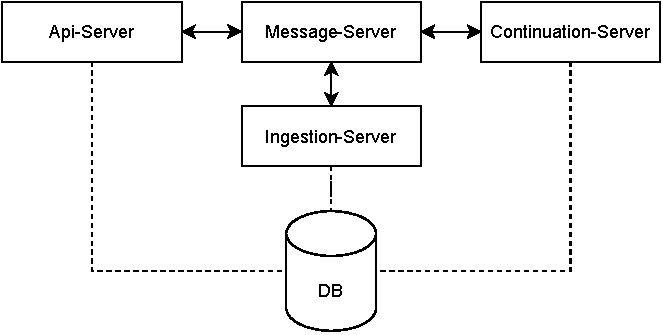
\includegraphics{Grafiken/ingestion-arch.pdf}
  \caption{Architektur der Ingestion Komponenten}
  \label{fig:ingestion_arch}
\end{figure}

\section{Plugins}


\section{Datenquellen}
Ein weiterer Kernpunkt der Ingestion-Schnittstelle ist die Modellierung der Datenquellen.
Zur Entwicklung eines Datenmodells für die Datenquellen, wird als erstes betrachtet, welcher verschiedenen Typen von Datenquellen möglich sind.
Danach wird unter Zuhilfenahme des Ergebnisses ein Modell entwickelt.
Das fertige Datenmodell enthält dann neben den für den Betrieb benötigten Informationen auch Daten über den Verlauf der Ingestion einer Datenquelle.
Um die Behebung von Fehlern bei einer Ingestion einfacher zu gestalten werden alle Überarbeitungen einer Datenquelle in Revisionen festgehalten.

\subsection{Datenquellen-Typen}
\label{sec:datasource-types}

Da das System alle möglichen Datenquellen unterstützen soll, werden hier mögliche Typen dargestellt, mit denen sich alle Datenquellen abdecken lassen.
Dazu werden Merkmale betrachtet die Struktur und Art der Ingestion bestimmen.
Die Struktur der verwendeten Daten ist entweder strukturiert, semi- oder unstrukturiert.
Da in der Vorarbeit, dem Masterprojekt, \textit{Apache Spark} verwendet wurde, ist dieser Punkt bereits abgedeckt und fällt bei der Entwicklung nicht weiter ins Gewicht.

Die Art der Datenquelle beschreibt, wie Daten in das System gelangen.
Dazu gibt es zwei Merkmale, in denen sich die Ingestions unterscheiden können.
Das erste ist die Unterscheidung zwischen Push- und Pull-Prinzip.
Bei dem Push-Prinzip werden die zu speichernden Daten in der Anfrage an das System gesendet und bei dem Pull-Prinzip muss dass System die Daten aus einer Quelle laden.
Die zweite Unterscheidung findet statt in einmalige in kontinuierliche Ingestion.
Diese Unterscheidungen können, müssen aber nicht, von der Datenquelle abhängig sein.
Als Beispiel gibt es Datenströme, die laufend Daten senden und somit eine Ingestion benötigen, die auch laufend Daten annimmt.
Im Gegensatz dazu gibt es Datenbanken, bei denen das System die Daten aus der Quelle laden muss und somit die Ingestion sowohl einmalig als auch kontinuierlich sein kann.

Es ergeben sich vier Verarbeitungswege bei der Ingestion, die in \fref{fig:ingestion_types} zu sehen sind.
Sowohl für Push- und Pull-Prinzip kann eine einfache Ingestion ausgeführt werden, die sich für kontinuierliche Pull-Ingestions wiederholt.
Bei einer kontinuierlichen Ingestion, bei der Daten an das System gesendet werden, handelt es sich um Datenströme, die eine extra Verarbeitung erfordern.

\begin{figure}
  \centering
  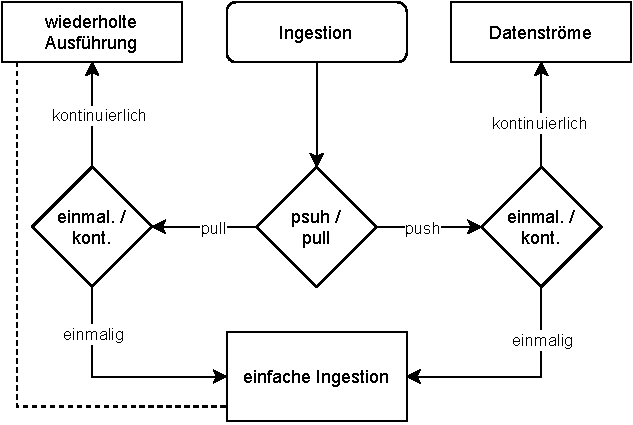
\includegraphics{Grafiken/ingestion-types.pdf}
  \caption{Ingestion-Typen}
  \label{fig:ingestion_types}
\end{figure}

\subsection{Datenquellen-Model}

Bei der Entwicklung des Datenmodells können die Informationen zur Datenquelle in drei Teilmodelle unterteilt werden.
Die \textbf{Revision} enthält alle veränderlichen Informationen über die Datenquelle und kann nur erstellt aber nicht geändert werden.
Ein \textbf{Ingestion-Event} beschreibt die Ausführung einer Ingestion.
Und in der \textbf{Datasource} werden sowohl alle statischen Informationen als auch die Listen von Revisionen und Ingestion-Events gespeichert.

Im folgenden werden die Felder der Datenmodelle beschrieben.
Falls eine Information direkt aus \textit{Apache Spark} abgeleitet ist, wird auch Angegeben an welcher Stelle diese angewendet wird.

\paragraph{Revision}
\subparagraph{Nummer}
Eine aufsteigende Nummer, die die Revision identifiziert.
Sie startet bei 0 und jede Nummer ist für eine Datenquelle einzigartig.
Gleichzeitig spiegelt die Nummer auch den zeitlichen Verlauf wieder.
\subparagraph{Erstellungsdatum}
Das Datum an dem die Revision erstellt wurde.
Da eine Revision nicht geändert werden kann, ist das Erstellungsdatum einer Revision auch das Änderungsdatum der dazugehörigen Datenquelle.
\subparagraph{Name}
Ein Name, der der Datenquelle im Datalake gegebn wird.
Dieser dient nur dazu die Datenquelle als Benutzer besser identifizieren zu können.
\subparagraph{ID Spalte}
Der Name der Spalte oder des Feldes, das einen Datensatz eindeutig identifiziert.
Die ID Spalte wird für die zuordnung der Datensätze bei der Deltaerkennung benötigt.
\subparagraph{Spark Abhägigkeiten}
Eine Liste von Abhängigkeiten, die der Spark Session bei der Ingestion mitgegeben wird.
Diese Liste entspricht der Option "`spark.jars.packages"' die bei der Erstellung einer Spark Session gestzt wird.
\subparagraph{Quelldateien}
Bei der Ingestion können die Daten über das Push-Prinzip in Form von Dateien an den Server gesendet werden.
Die Liste der Quelldateien enthält die Pfade zu diesen Dateien.
\subparagraph{Typ beim Lesen}
Der Typ der zu lesenden Daten, wie in \ref{sec:datasource-types} beschrieben.
\subparagraph{Format beim Lesen}
Das Format in dem die Daten gelesen werden sollen.
Der Wert aus diesem Feld wird bei der Ingestion über die \verb|format| Methode eines Readers gesetzt.
\subparagraph{Optionen beim Lesen}
Eine Liste von Schlüssel-Wert-Paaren, die als Optionen des Readers in \textit{Apache Spark} gesetzt werden.
Über diese wird die verbindung zur Datenquelle definiert.
\subparagraph{Aktualisierung für Datenquelle}
Es kann für einen Datenquelle festgelegt werdne, dass diese Aktualisierungen für eine andere enthält.
Das ermöglicht die Nutzung von eigenen Change Data Capture Lösungen.
Dabei muss die Datenquelle aber dem internet Change Data Format entsprechen.
\subparagraph{Typ beim Schreiben}
Der Typ für das Schreiben der Daten legt fest, ob intern mit Versionierung oder in einen freien Speicher geschrieben werden soll.
\subparagraph{Format und Optionen beim Schreiben}
Das Format und die Optionen beim Schreiben funktionieren analog zu denen beim Lesen.
Sie werden jedoch nicht beim Reader gesetzt sondern beim Writer.
Gerade bei Datenströmen muss darauf geachtet werden, dass nicht in jedem Format ein Datenstrom geschrieben werden kann.
\subparagraph{Schreibmodus}
Der Modus in dem die Daten geschrieben werden.
Die Auswahlmöglichkeiten werden auch durch \textit{Apache Spark} festegelegt.
\subparagraph{Zeitsteuerungen}
Eine Liste die festlegt, zu welchen Zeitpunkte eine Ingestion der Datenquelle asugeführt werden soll.
\subparagraph{Plugin Abhängigkeiten}
Eine Liste von Abhängigkeiten, die von den Plugins der Datenquelle benötigt werden.
\subparagraph{Plugins}
Die Speicherorte der Plugins.

\paragraph{Ingestion-Event}
\subparagraph{Nummer}
Die Nummer um ein Ingestion-Event zu identifizieren.
Sie funktioniert genau wie die Nummer der Revisions.
\subparagraph{Status}
Der aktuelle Status in dem sich das Event befindet.
Er gibt auskunft, ob die Ingestion gestartet wurde, gerade läuft oder beendet wurde.
\subparagraph{Revisionsnummer}
Die Nummer der Revision, mit der die Inegstion gestartet wurde.
Mit Hilfe der Revisionsnummer ist es leichter Fehler in der Ingestion zu finden und zu beheben.
\subparagraph{Start- und Endzeit}
Die Zeitpunkte des Starts und Endes eines Ingestion-Durchlaufs.
Wenn die Ingestion noch in der Asuführung ist, ist keine Endzeit gesetzt.
\subparagraph{Fehler}
Die Fehlerausgabe, wenn die Ingestion nicht erfolgreich ausgeführt werden konnte.

\paragraph{Datasource}
\subparagraph{ID}
Eine Identifikationsnummer, die für jede Datenquelle eindeutig ist.
\subparagraph{Aktuelle Revision}
Die Nummer der aktuellen Revision.
Neue Ingestions werden mit den Informationen aus dieser Revision ausgeführt.
\subparagraph{Alle Revisionen}
Eine Liste aller Revisionen.
\subparagraph{Letzte Ingestion}
Die Nummer des zuletzt gestarteten Ingestion-Durchlaufs.
\subparagraph{Letzte erfolgreiche Ingestion}
Die Nummer des letzten erfolgreich abgeschlossenen Ingestion-Durchlauf.
\subparagraph{Alle Ingestion-Events}
Eine Liste aller Ingestion Events.

\section{Ingestion}
Bei der Entwicklung der Ingestion wird das Laden der Daten und die Architektur der Anwendung betrachtet.
Es wird eine Datenmodell, in dem die Informationen zu den Datenquellen gespeichert werden, der Ablauf der verschiedenen Ingestion-Prozesse und die Kommunikation zwischen den einzelnen Mircoservices entwickelt.

\subsection{Server Architektur}

Für die Umsetzung der Mircoservice-Architektur wird die Ingestion in Komponenten aufgeteilt, die \fref{fig:ingestion_arch} zu sehen sind.
Es gibt drei Services, die für die Ingestion spezifischen Aufgaben zuständig sind, eine Datenbank, in der die Informationen über Datenquellen gespeichert werden und einen Service, der für die Kommunikation verantwortlich ist.
Der \textbf{Api-Server} bietet einen REST-Schnittstelle, über die man mit der Ingestion interagieren kann.
Hier werden die Endpunkte aus \fref{tab:enpoints} benötigt, die die Schnittstellen zur Verwaltung von Datenquellen und das Ausführen von Ingestions bereitstellen.
Außerdem ist er dafür zuständig, die empfangenen Informationen über Datenquellen in der Datenbank zu verwalten.
der \textbf{Continuation-Server} überprüft regelmäßig alle kontinuierlichen Datenquellen, ob diese eine Zeitsteuerung haben und aktuell ausgeführt werden sollten.
Der \textbf{Ingestion-Server} ist die Anwendung, die die eigentliche Ingestion ausführt.
Dafür wartet dieser auf eine Aufforderung durch entweder den Api- oder den Continuation-Server.

\begin{table}[!ht]
  \centering
  \begin{tabular}{| l | l | p{3in} |}
    \hline
    Pfad                                      & HTTP-Methode & Beschreibung                                                          \\
    \hline \hline
    /datasources                              & GET          & Liefert alle im System gespeicherten Datenquellen                     \\
    \hline
    /datasources/\textless id\textgreater     & GET          & Liefert die Datenquelle mit der im Pfad übergebenen Id                \\
    \hline
    /datasources                              & POST         & Erstellt eine neue Datenquelle                                        \\
    \hline
    /datasources/\textless id\textgreater     & PUT          & Bearbeitet die Daten Datenquelle mit der im Pfad übergebenen Id       \\
    \hline
    /datasources/\textless id\textgreater/run & GET          & Startet eine Ingestion der Datenquelle mit der im Pfad übergebenen Id \\
    \hline
  \end{tabular}
  \caption{Endpunkte des Api-Servers}
  \label{tab:enpoints}
\end{table}

\subsection{Plugins}
Da bei manchen Ingestions nicht immer ein festgelegtes Vorgehen ausreicht, um die Daten aus bestimmten Datenqellen zu laden, muss ein System entwickelt werden, wie möglichst ohne großen Aufwand die Inegstion erweitert werden kann.
Beispiele für solche Fälle sind die Verarbeitung von Datenströmen oder die Ingestion von Daten aus APIs, die nicht generallisiert werden können.
Als Lösung für das Problem, können Plugins der Datenquelle hinzugefügt werden.
Diese Plugins sollen Logik enthalten, die an verschiedenen Stellen der Ingestion ausgeführt werden sollen.
Aktuell sind diese Stellen das Laden der Daten, nach dem Laden der Daten und die Stream-Verarbeitung.
Dabei ist zu beachten, dass Plugins, die das Laden der Daten abhandeln, das Standardverhalten des Ingestion-Servers überschreiben und das Stream-Verarbeitung nur mit Plugins möglich ist.
Damit es nicht zu Konflikten bei Abhängigkeiten der Plugins gibt, muss der Ingestion-Server eine Mechanik implementieren, bei der die Abhängigkeiten der Plugins für jede Datenquelle dynamisch gealden werden.


\section{Deltaerkennung}

\chapter{Umsetzung}

Bei der Umsetzung ist die erste Frage, die zu klären ist, mit welcher Programmiersprache gearbeitet werden soll.
In diesem habe ich mich aus verschiedenen Gründen für \textit{Python} entschieden.
Der erste ist, dass \textit{Python} bereits im Masterprojekt verwendet wurde und so die Integration leichter fällt.
Als zweites geht es speziell um die Bibliothek \textit{PySpark}.
\textit{PySpark} ist die Bibliothek, mit deren Hilfe \textit{Apache Spark} in \textit{Python} verwendet werden kann.
Neben \textit{PySpark} gibt es auch Bibliotheken für die Sprachen \textit{Java} und \textit{Scala}.
Der entscheidende Unterschied hierbei ist aber, dass \textit{Python} eine interpretierte Sprache ist.
Das bedeutet, dass der geschrieben Programmcode nicht in Maschinensprache übersetzt wird, sondern durch einen sogenannten Interpreter ausgeführt.
In diesem Anwendungsfall hat das den Vorteil, dass die Spark-Jobs nicht als kompilierte jar-Datei explizit ausgeführt werden müssen, sondern der Interpreter sich an den entsprechenden Zeitpunkten um die Ausführung kümmert.
Das bedeutet, dass die Konfiguration eines Spark-Jobs dynamisch während der Ausführung des Programms gemacht werden kann und man so mehr Freiheit für die Entwicklung bekommt.
Der letzte Vorteil ist, dass Programmcode dynamisch aus Dateien nachgeladen werden kann, was für die Umsetzung der Plugins wichtig ist.

\section{Voraussetzungen}
Um das Datalake System umsetzen zu können müssen einige Voraussetzungen erfüllt sein.
Die erste ist, wie in \ref{fig:ingestion_arch} bereits beschrieben, dass ein Server benötigt wird, der sich um die Verteilung von Nachrichten kümmert.
Als zweites muss außerdem ein zentraler Speicher für Dateien bereit stehen, indem sowohl Datenquelldateien als auch Plugindateien abgelet und von jedem Server abgerufen werden können.

\subsection{Apache Kafka}

\textit{Apache Kafka} ist ein verteiltes Event-Streaming-System, dass nach dem Publish-Subscribe-Muster funktioniert.
Events können von Produzenten in das System veröffentlicht werden und Konsumenten können diese Events abonnieren.
Das ganze läuft dabei in Echtzeit ab.
Durch seine Verteilung kann \textit{Kafka} den Ausfall einzelner Server ausgleichen.
Außerdem können Ströme von Events für einen beliebigen Zeitraum abgespeichert werden.

\textit{Kafka} besteht aus einem Cluster von Servern und verschiedenen Clients.
Es gibt zwei Arten von Servern.
Einige bilde die Speicherebene von \textit{Kafka} und werden Broaker genannt.
Die anderen verwenden \textbf{Kafka Connect}\footnote{https://kafka.apache.org/documentation/\#connect} um extierende Systeme, zum Beipsiel eine Datenbank, in das Kafka Cluster zu integrieren.
Anwendungen, die entweder Events produzieren oder konsumieren sind die Clients.

In diesem System repräsentiert ein Event den Fakt, dass etwas "`passiert"' ist und besteht aus einem Schlüssel, einem Wert, einem Zeitstempel und optionalen Metadaten.
Dabei werden die Werte nicht interpretiert sonder einfach als Block versendet und können so bliebige Struktur haben.
Events werden in sogenannte Topics unterteilt.
Es kann immer mehrere Produzenten oder Konsumenten auf einer Topic geben.
Events in einer Topic können mehrfach gelesen werden und werden nicht nach dem Konsumieren gelöscht.
Es kann aber für jede Topic einzeln eine Dauer festgelegt werden, nach der die Events verworfen werden.
Um eine Topic fehlertolerant zu machen, kann diese replziert werden.

Topics werden in Partitionen über verschiedene Broaker aufgeteilt, so dass das ganze System gut skalierbar wird.
Ein Produzenten kann zum Beispiel Events auf mehreren Broakern gleichzeitig veröffentlichen.
Wenn ein Event in einer Topic veröffentlicht wird, wird dieses an eine der Partitionen angehängt.
Events, die den gleichen Schlüssel haben werden immer der gleichen Partition zugeordnet und Events einer Partition kommen garantiert in der Reihenfolge des Schreibens bei dem Konsumenten der Partition an \parencite{kafka-docs}.

\textit{Apache Kafka} wird im Big Data Bereich weit verbreitet um Datenströme zu verarbeiten.
Daher macht es Sinn, \textit{Kafka} auch in dieses Data Lake System zu integrieren und darin bereit zu stellen.
Außerdem kann es auch für die Kommunikation zwischen den verschiedenen Microservices verwendet werden.

\subsection{Hadoop Distributed File System}

Als Speicher wird das \textit{Hadoop Distributed File System (HDFS)} verwendet.
Das \textit{HDFS} ist ein verteiltes, auf große Dateien ausgelegtes Dateisystem.
Ein \textit{HDFS} Cluster besteht aus einem Namenode und mehreren Datanodes.

Der Namenode verwaltet den Baum des Dateisystems und kontrolliert den Zugriff durch Clients.
Zusätzlich führt er Operation auf dem Dateisystem aus.
Dazu zählen das Öffnen, Schließen oder Umbenennen von Dateien oder Ordnern.
Die Dateien selbst werden in Blöcke aufgeteilt auf den Datanodes gespeichert.
Diese sind auch dafür verantwortlich, Lese- und Schreibanfragen zu bedienen und verwalten die Erstellung, Löschung und Replikation unter Anleitung des Namenodes \parencite{hdfs}.

Das \textit{HDFS} ist ebenfalls eine weit verbreitete Technik im Big Data Bereich und eignet sich auch hier, durch die Auslegung auf große Dateien, sehr gut um die Quelldateien der Datenquellen abzulegen.
Außerdem sind Dateien auf allen Servern verfügbar, da es sowohl eine REST-Schnittstelle als auch Unterstützung in \textit{Apache Spark} gibt.

\section{Ingestion}

\subsection{Datenquelle}

Bei der Implementierung 

\begin{figure}
    \centering
    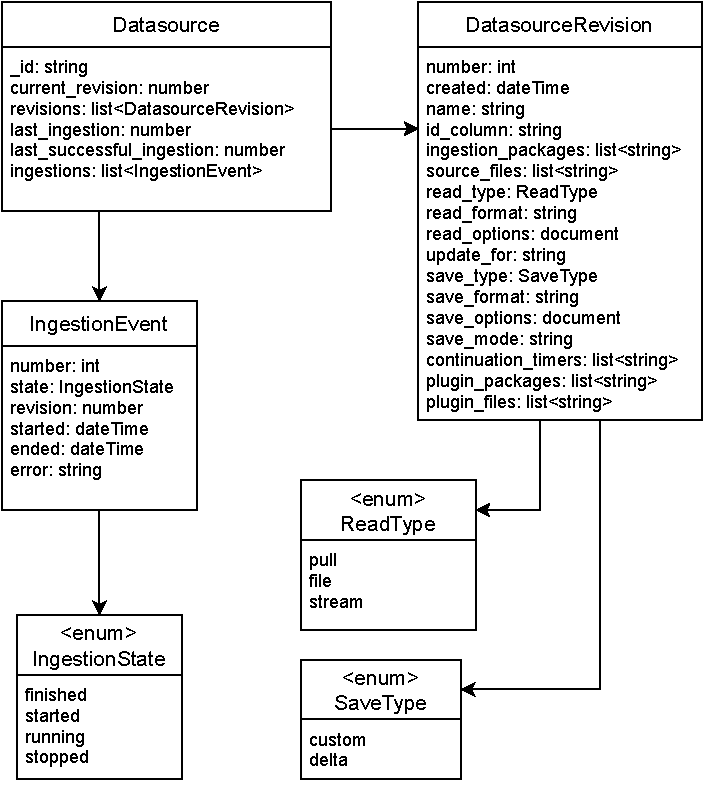
\includegraphics{Grafiken/ingestion-Datamodel.pdf}
    \caption{Datenmodell der Datenquelle}
    \label{fig:datasource_model}
\end{figure}

\subsection{Api-Server}

Da auch das Masterprojekt eine REST-Schnittstelle hat, bietet es sich an, diesen Server so zu erweitern, dass er als Api-Server für das neue System fungiert.
Um die neuen Endpunkte in die aktuelle Lösung zu integrieren, werden die existierenden Pfade, bis auf die zur Authentifizierung, nach "`/api/v1/"' verschoben und die neuen unter "`/api/v2/"' eingefügt.
Auf Grund der Tatsache, dass das neue System mit einem eigenen Datenmodell arbeitet, ist damit die Integration bereits abgehandelt, es muss nur darauf geachtet werden, die Funktionen der beiden Versionen zu trennen.
Die Endpunkte werden mit ihren Funktionen, wie in \fref{sec:arch} beschrieben, implementiert.

Bei der Erstellung und dem Aktualisieren von Datenquellen werden jedes mal eine neue Revision 
Dabei muss besonders darauf geachtet werden, dass bei jeder Änderung einer \verb|Datasource| eine neue \verb|DatasourceRevision| angelegt wird.
Die Quell- oder Plugindateien werden zentral im \textit{HDFS} jeweils einem Unterordner pro Datenquelle abgelegt.
So sind die Dateien von überall aus erreichbar und können auch bei replizierten oder verteilten Microservices verwendet werden.


\subsection{Ingestion-Server}



\subsection{Continuation-Server}

\section{Deltaerkennung}

\section{Datenversionierung}


\newpage
% \bibliographystyle{unsrtnat}
% \bibliography{literatur}

\printbibliography

\end{document}
